\documentclass{standalone}
\usepackage{tikz}
\usetikzlibrary{patterns, positioning}
\usepackage[sfdefault]{ClearSans} %% option 'sfdefault' activates Clear Sans as the default text font
\usepackage[T1]{fontenc}

\begin{document}
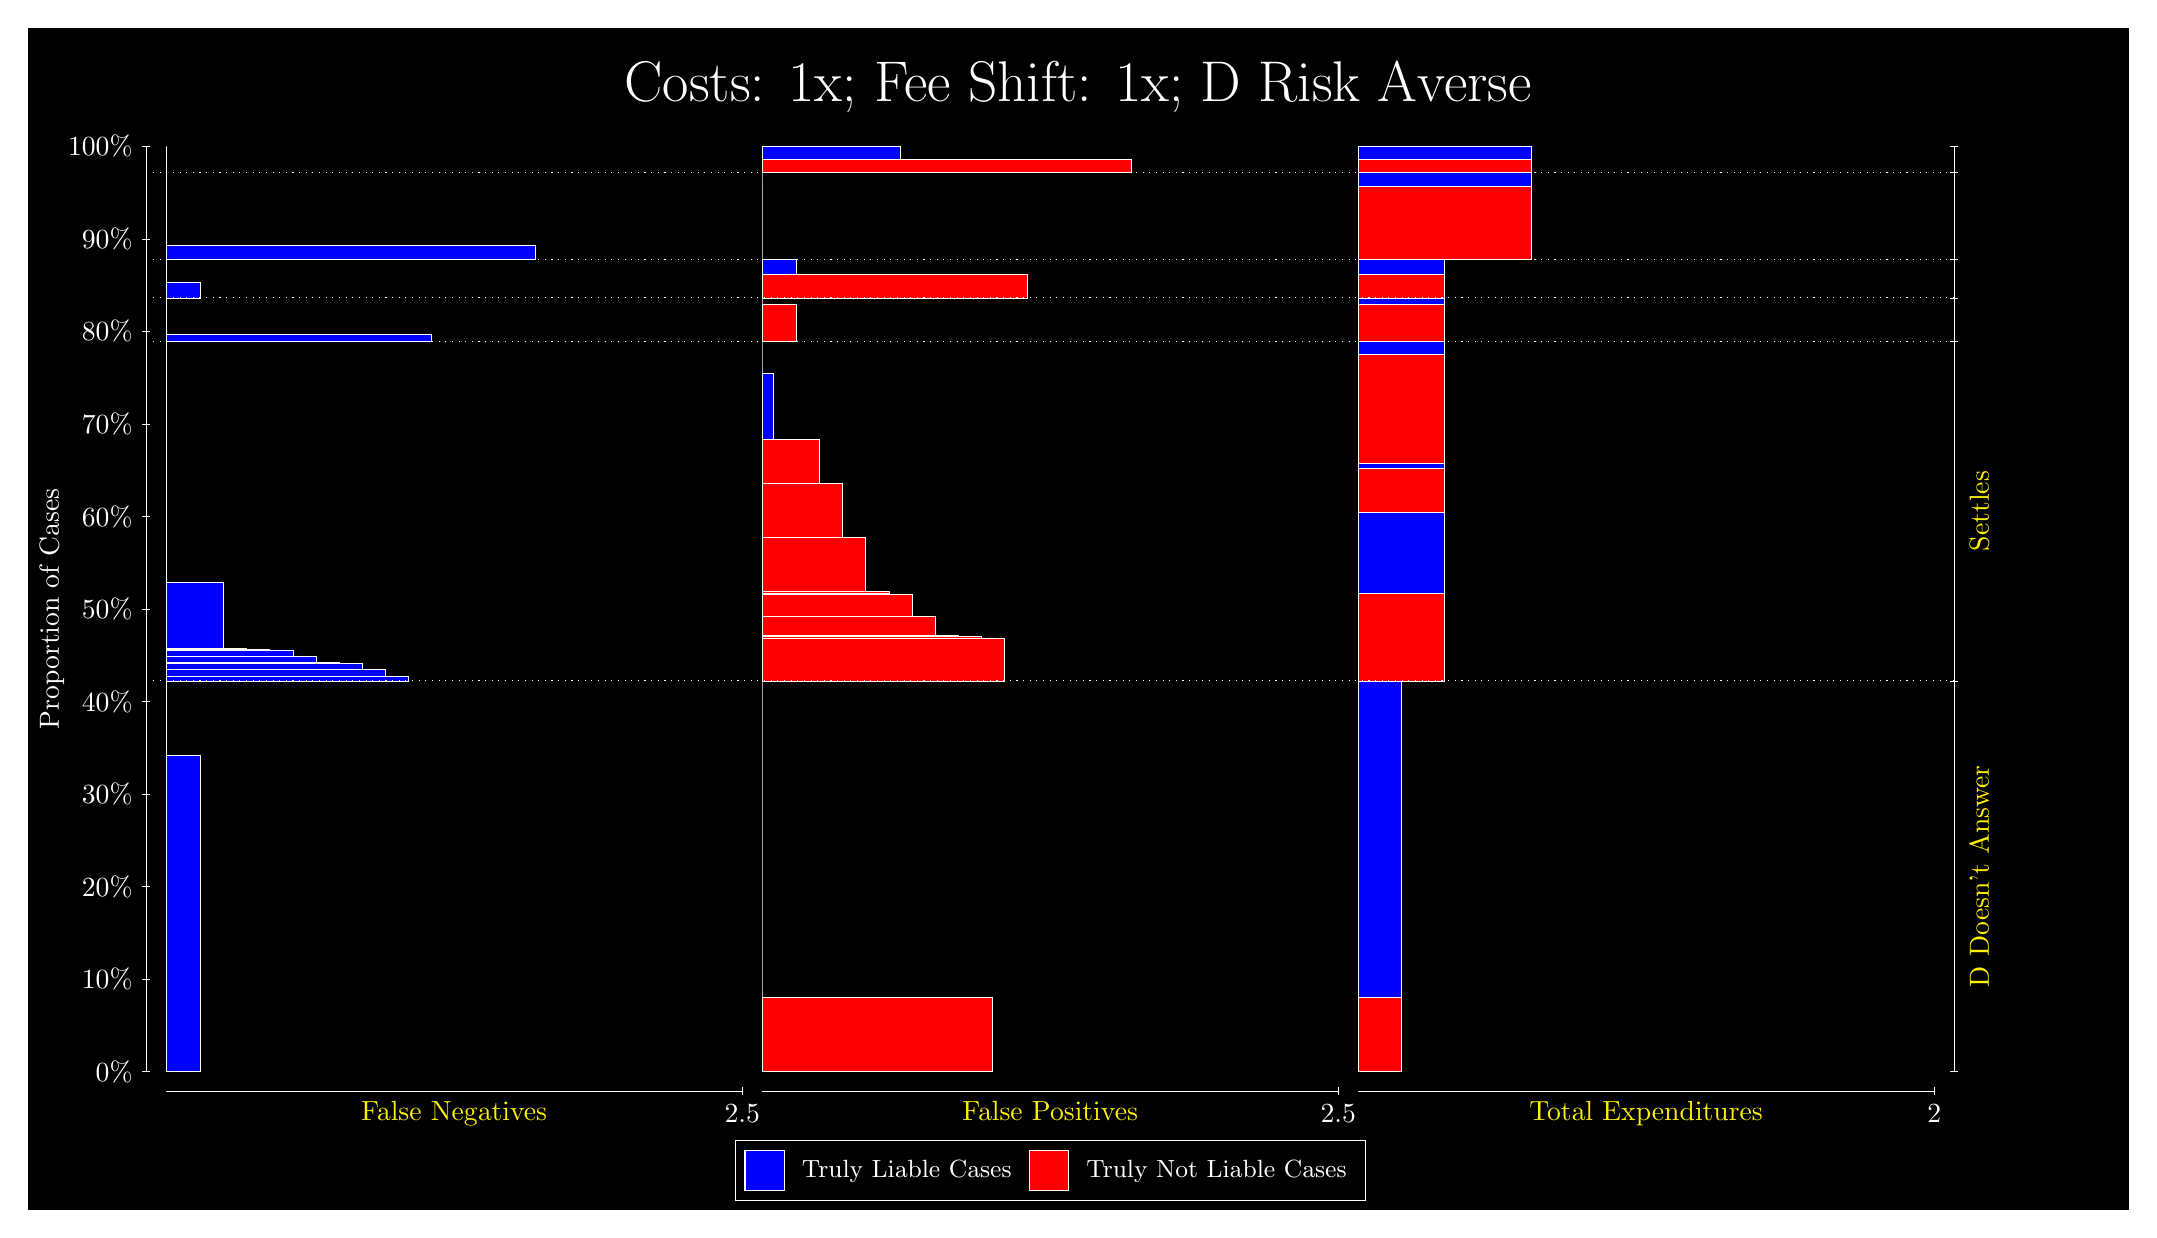
\begin{tikzpicture}
\draw[fill=black] (0,0) rectangle (26.667,15);
\draw[text=white] (0,13.5) rectangle (26.667,15) node[midway] {\huge Costs: 1x; Fee Shift: 1x; D Risk Averse};
\draw[white, very thin] (1.5,1.75) -- (1.5,13.5);
\node[rotate=90, text=white, anchor=center] at (0.3, 7.625) {Proportion of Cases};
\draw[white, very thin] (1.45,1.75) -- (1.55,1.75);
\node[text=white, anchor=east] at (1.45, 1.75) {0\%};
\draw[white, very thin] (1.45,2.925) -- (1.55,2.925);
\node[text=white, anchor=east] at (1.45, 2.925) {10\%};
\draw[white, very thin] (1.45,4.1) -- (1.55,4.1);
\node[text=white, anchor=east] at (1.45, 4.1) {20\%};
\draw[white, very thin] (1.45,5.275) -- (1.55,5.275);
\node[text=white, anchor=east] at (1.45, 5.275) {30\%};
\draw[white, very thin] (1.45,6.45) -- (1.55,6.45);
\node[text=white, anchor=east] at (1.45, 6.45) {40\%};
\draw[white, very thin] (1.45,7.625) -- (1.55,7.625);
\node[text=white, anchor=east] at (1.45, 7.625) {50\%};
\draw[white, very thin] (1.45,8.8) -- (1.55,8.8);
\node[text=white, anchor=east] at (1.45, 8.8) {60\%};
\draw[white, very thin] (1.45,9.975) -- (1.55,9.975);
\node[text=white, anchor=east] at (1.45, 9.975) {70\%};
\draw[white, very thin] (1.45,11.15) -- (1.55,11.15);
\node[text=white, anchor=east] at (1.45, 11.15) {80\%};
\draw[white, very thin] (1.45,12.325) -- (1.55,12.325);
\node[text=white, anchor=east] at (1.45, 12.325) {90\%};
\draw[white, very thin] (1.45,13.5) -- (1.55,13.5);
\node[text=white, anchor=east] at (1.45, 13.5) {100\%};

\draw[white, very thin] (24.457,1.75) -- (24.457,13.5);
\draw[white, very thin] (24.407,1.75) -- (24.507,1.75);
\node[anchor=west] at (24.407, 1.75) {};
\draw[white, very thin] (24.407,6.7119) -- (24.507,6.7119);
\node[anchor=west] at (24.407, 6.7119) {};
\draw[white, very thin] (24.407,11.024) -- (24.507,11.024);
\node[anchor=west] at (24.407, 11.024) {};
\draw[white, very thin] (24.407,11.575) -- (24.507,11.575);
\node[anchor=west] at (24.407, 11.575) {};
\draw[white, very thin] (24.407,12.067) -- (24.507,12.067);
\node[anchor=west] at (24.407, 12.067) {};
\draw[white, very thin] (24.407,13.171) -- (24.507,13.171);
\node[anchor=west] at (24.407, 13.171) {};
\draw[white, very thin] (24.407,13.5) -- (24.507,13.5);
\node[anchor=west] at (24.407, 13.5) {};

\draw[white, very thin, fill=blue] (1.75,1.75) rectangle (2.1891,5.7659);
\draw[white, very thin, fill=red] (1.75,5.7659) rectangle (1.75,6.7119);
\draw[white, very thin, fill=blue] (1.75,6.7119) rectangle (4.8239,6.7746);
\draw[white, very thin, fill=blue] (1.75,6.7746) rectangle (4.5312,6.8544);
\draw[white, very thin, fill=blue] (1.75,6.8544) rectangle (4.2384,6.9341);
\draw[white, very thin, fill=blue] (1.75,6.9341) rectangle (3.9457,6.9413);
\draw[white, very thin, fill=blue] (1.75,6.9413) rectangle (3.6529,7.0253);
\draw[white, very thin, fill=blue] (1.75,7.0253) rectangle (3.3602,7.1013);
\draw[white, very thin, fill=blue] (1.75,7.1013) rectangle (3.0674,7.1126);
\draw[white, very thin, fill=blue] (1.75,7.1126) rectangle (2.7746,7.1235);
\draw[white, very thin, fill=blue] (1.75,7.1235) rectangle (2.4819,7.9589);
\draw[white, very thin, fill=red] (1.75,7.9589) rectangle (1.75,11.024);
\draw[white, very thin, fill=blue] (1.75,11.024) rectangle (5.1167,11.107);
\draw[white, very thin, fill=red] (1.75,11.107) rectangle (1.75,11.575);
\draw[white, very thin, fill=blue] (1.75,11.575) rectangle (2.1891,11.771);
\draw[white, very thin, fill=red] (1.75,11.771) rectangle (1.75,12.067);
\draw[white, very thin, fill=blue] (1.75,12.067) rectangle (6.4341,12.24);
\draw[white, very thin, fill=red] (1.75,12.24) rectangle (1.75,13.171);
\draw[white, very thin, fill=red] (1.75,13.171) rectangle (1.75,13.34);
\draw[white, very thin, fill=blue] (1.75,13.34) rectangle (1.75,13.5);
\draw[white, very thin, fill=red] (9.3189,1.75) rectangle (12.246,2.6959);
\draw[white, very thin, fill=blue] (9.3189,2.6959) rectangle (9.3189,6.7119);
\draw[white, very thin, fill=red] (9.3189,6.7119) rectangle (12.393,7.2519);
\draw[white, very thin, fill=red] (9.3189,7.2519) rectangle (12.1,7.2719);
\draw[white, very thin, fill=red] (9.3189,7.2719) rectangle (11.807,7.2935);
\draw[white, very thin, fill=red] (9.3189,7.2935) rectangle (11.515,7.533);
\draw[white, very thin, fill=red] (9.3189,7.533) rectangle (11.222,7.8053);
\draw[white, very thin, fill=red] (9.3189,7.8053) rectangle (10.929,7.8256);
\draw[white, very thin, fill=red] (9.3189,7.8256) rectangle (10.929,7.8488);
\draw[white, very thin, fill=red] (9.3189,7.8488) rectangle (10.636,8.5314);
\draw[white, very thin, fill=red] (9.3189,8.5314) rectangle (10.344,9.2156);
\draw[white, very thin, fill=red] (9.3189,9.2156) rectangle (10.051,9.7769);
\draw[white, very thin, fill=blue] (9.3189,9.7769) rectangle (9.4652,10.612);
\draw[white, very thin, fill=blue] (9.3189,10.612) rectangle (9.3189,11.024);
\draw[white, very thin, fill=red] (9.3189,11.024) rectangle (9.758,11.492);
\draw[white, very thin, fill=blue] (9.3189,11.492) rectangle (9.3189,11.575);
\draw[white, very thin, fill=red] (9.3189,11.575) rectangle (12.686,11.871);
\draw[white, very thin, fill=blue] (9.3189,11.871) rectangle (9.758,12.067);
\draw[white, very thin, fill=red] (9.3189,12.067) rectangle (9.3189,12.998);
\draw[white, very thin, fill=blue] (9.3189,12.998) rectangle (9.3189,13.171);
\draw[white, very thin, fill=red] (9.3189,13.171) rectangle (14.003,13.34);
\draw[white, very thin, fill=blue] (9.3189,13.34) rectangle (11.075,13.5);
\draw[white, very thin, fill=red] (16.888,1.75) rectangle (17.437,2.6959);
\draw[white, very thin, fill=blue] (16.888,2.6959) rectangle (17.437,6.7119);
\draw[white, very thin, fill=red] (16.888,6.7119) rectangle (17.986,7.8256);
\draw[white, very thin, fill=blue] (16.888,7.8256) rectangle (17.986,8.8466);
\draw[white, very thin, fill=red] (16.888,8.8466) rectangle (17.986,9.4079);
\draw[white, very thin, fill=blue] (16.888,9.4079) rectangle (17.986,9.4706);
\draw[white, very thin, fill=red] (16.888,9.4706) rectangle (17.986,10.861);
\draw[white, very thin, fill=blue] (16.888,10.861) rectangle (17.986,11.024);
\draw[white, very thin, fill=red] (16.888,11.024) rectangle (17.986,11.492);
\draw[white, very thin, fill=blue] (16.888,11.492) rectangle (17.986,11.575);
\draw[white, very thin, fill=red] (16.888,11.575) rectangle (17.986,11.871);
\draw[white, very thin, fill=blue] (16.888,11.871) rectangle (17.986,12.067);
\draw[white, very thin, fill=red] (16.888,12.067) rectangle (19.083,12.998);
\draw[white, very thin, fill=blue] (16.888,12.998) rectangle (19.083,13.171);
\draw[white, very thin, fill=red] (16.888,13.171) rectangle (19.083,13.34);
\draw[white, very thin, fill=blue] (16.888,13.34) rectangle (19.083,13.5);
\draw[white, dotted] (1.5,6.7119) -- (24.457,6.7119);
\draw[white, dotted] (1.5,11.024) -- (24.457,11.024);
\draw[white, dotted] (1.5,11.575) -- (24.457,11.575);
\draw[white, dotted] (1.5,12.067) -- (24.457,12.067);
\draw[white, dotted] (1.5,13.171) -- (24.457,13.171);
\draw[white, very thin] (1.75,1.5) -- (9.0689,1.5);
\node[text=yellow, anchor=north] at (5.4094, 1.5) {False Negatives};
\draw[white, very thin] (9.0689,1.45) -- (9.0689,1.55);
\node[text=white, anchor=north] at (9.0689, 1.45) {2.5};

\draw[white, very thin] (9.3189,1.5) -- (16.638,1.5);
\node[text=yellow, anchor=north] at (12.978, 1.5) {False Positives};
\draw[white, very thin] (16.638,1.45) -- (16.638,1.55);
\node[text=white, anchor=north] at (16.638, 1.45) {2.5};

\draw[white, very thin] (16.888,1.5) -- (24.207,1.5);
\node[text=yellow, anchor=north] at (20.547, 1.5) {Total Expenditures};
\draw[white, very thin] (24.207,1.45) -- (24.207,1.55);
\node[text=white, anchor=north] at (24.207, 1.45) {2};

\node[text=yellow, centered, rotate=90] at (24.777, 4.2309) {D Doesn't Answer};
\node[text=yellow, centered, rotate=90] at (24.777, 8.8679) {Settles};





\draw (12.978300999999998,1.5) node[draw=none] (baseCoordinate) {};
\begin{scope}[align=center]
        \matrix[scale=0.5, draw=white, below=0.5cm of baseCoordinate, nodes={draw}, column sep=0.1cm]{
            \node[rectangle, draw, minimum width=0.5cm, minimum height=0.5cm, fill=blue] {}; &
            \node[draw=none, font=\small, text=white] (B) {Truly Liable Cases}; &
            \node[rectangle, draw, minimum width=0.5cm, minimum height=0.5cm, fill=red] {}; &
            \node[draw=none, font=\small, text=white] (B) {Truly Not Liable Cases}; \\
            };
\end{scope}

\end{tikzpicture}
\end{document}